\documentclass[a4paper,12pt]{article}

\usepackage{amssymb}
\usepackage{amsmath}
\usepackage{amsfonts}
\usepackage{txfonts}
\usepackage{upgreek}
\usepackage{graphicx}
\usepackage{siunitx}
\usepackage{enumerate}
\usepackage[left=2cm,right=2cm,top=2cm,bottom=2cm]{geometry}

\usepackage[obeyspaces]{url}

%\newcommand{\question}[2]{\textbf{\textit{#1}}\quad{\footnotesize\textit{(#2 points)}}\\[3mm]}
\newcommand{\question}[1]{\textbf{\textit{#1}}}
\newcommand{\points}[1]{\quad{\footnotesize\textit{(#1 points)}}}
\newcommand{\point}{\quad{\footnotesize\textit{(1 point)}}}
\newcommand{\HRule}{\rule{\linewidth}{0.3mm}}
\newcommand{\dd}{\mathrm{d}}
\renewcommand{\pi}{\uppi}
\newcommand{\ii}{\mathrm{i}}
\renewcommand{\thefootnote}{\normalsize\fnsymbol{footnote}}
\DeclareMathOperator{\e}{e}
\newcommand{\bra}{\langle}
\newcommand{\ket}{\rangle}

\renewcommand{\theequation}{\Roman{equation}}

\begin{document}
\pagestyle{empty}

\begin{center}
\LARGE \textbf{Astronomy from 4 perspectives: the Dark Universe}
\HRule
\end{center}
\begin{flushright}
prepared by: Heidelberg participants and BMS
\end{flushright}
\begin{center}
{\Large \textbf{play with data: virial theorem and periodic motion}}
\end{center}
\vspace{5mm}

\noindent
In these exercises we will explore the virial theorem by solving equations of motions numerically and measuring averaged energies from the solutions.

\begin{enumerate}[\itshape \bfseries 1.]

\item \question{virial theorem and the harmonic oscillator}\\
The script \path{harmonic.py} generates a solution to the harmonic oscillator equation $\ddot{x} = -x$ by transforming it with the definition $y=\dot{x}$ into a coupled first order equation,
\begin{equation}
\frac{\dd}{\dd t}
\left(
\begin{array}{c}
x\\
y
\end{array}
\right)
=
\left(
\begin{array}{cc}
0 & 1\\
-1 & 0
\end{array}
\right)
\left(
\begin{array}{c}
x\\
y
\end{array}
\right),
\end{equation}
where the angular frequency is set to $\omega=1$ for the numerics.
\begin{enumerate}[(a)]
\item{Is the total energy conserved?}
\item{Please run the script and measure the average kinetic and potential energies: Do you find $\bra T\ket = \bra V\ket$ for the harmonic oscillator?}
\item{Is $\bra T\ket = \bra V\ket$ true for any initial condition?}
\end{enumerate}

\begin{figure}[h]
\begin{center}
\resizebox{7.5cm}{!}{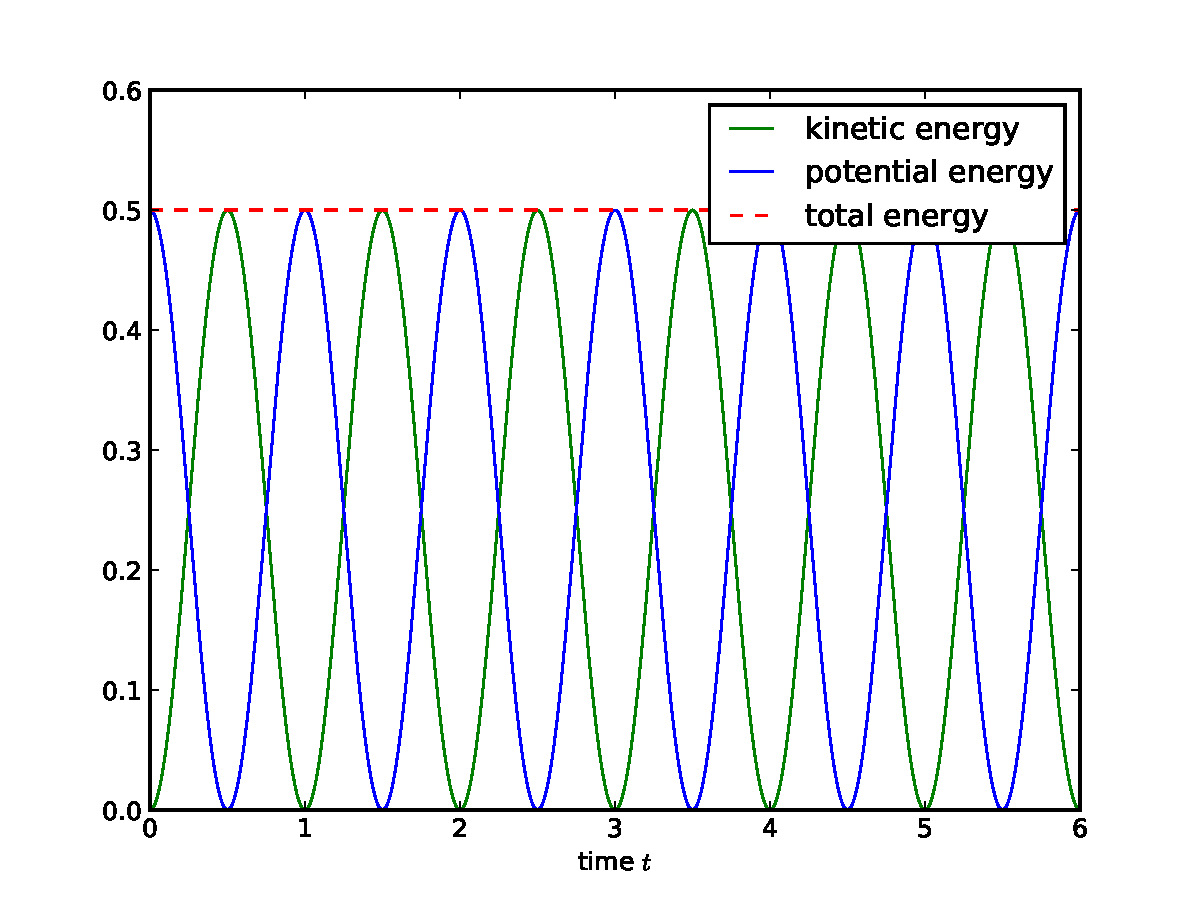
\includegraphics{./figures/harmonic.pdf}}
\caption{numerical solutions to the harmonic oscillator}
\end{center}
\end{figure}


\item \question{virial relationship in the anharmonic oscillator}\\
The virial theorem makes a prediction for the average kinetic and potential energies in any system with a scale-free potential, for instance the anharmonic oscillator with the potential $\Phi\propto x^{2n}$. The script \path{anharmonic.py} solves the equation of motion. The constant of proportionality is set to 1.
\begin{enumerate}[(a)]
\item{What's the equation of motion for the potential $\Phi=x^{2n}/(2n)$, and what's the corresponding coupled first order system?}
\item{Why are there with increasing $n$ phases of constant velocity and a sawtooth pattern in position?}
\item{Please measure the average kinetic and potential energies over many oscillations: What's their ratio $r$ as a function of $n$? Why does $r=\bra T\ket/\bra V\ket$ increase with $n$?}
\end{enumerate}

\begin{figure}[h]
\begin{center}
\resizebox{7.5cm}{!}{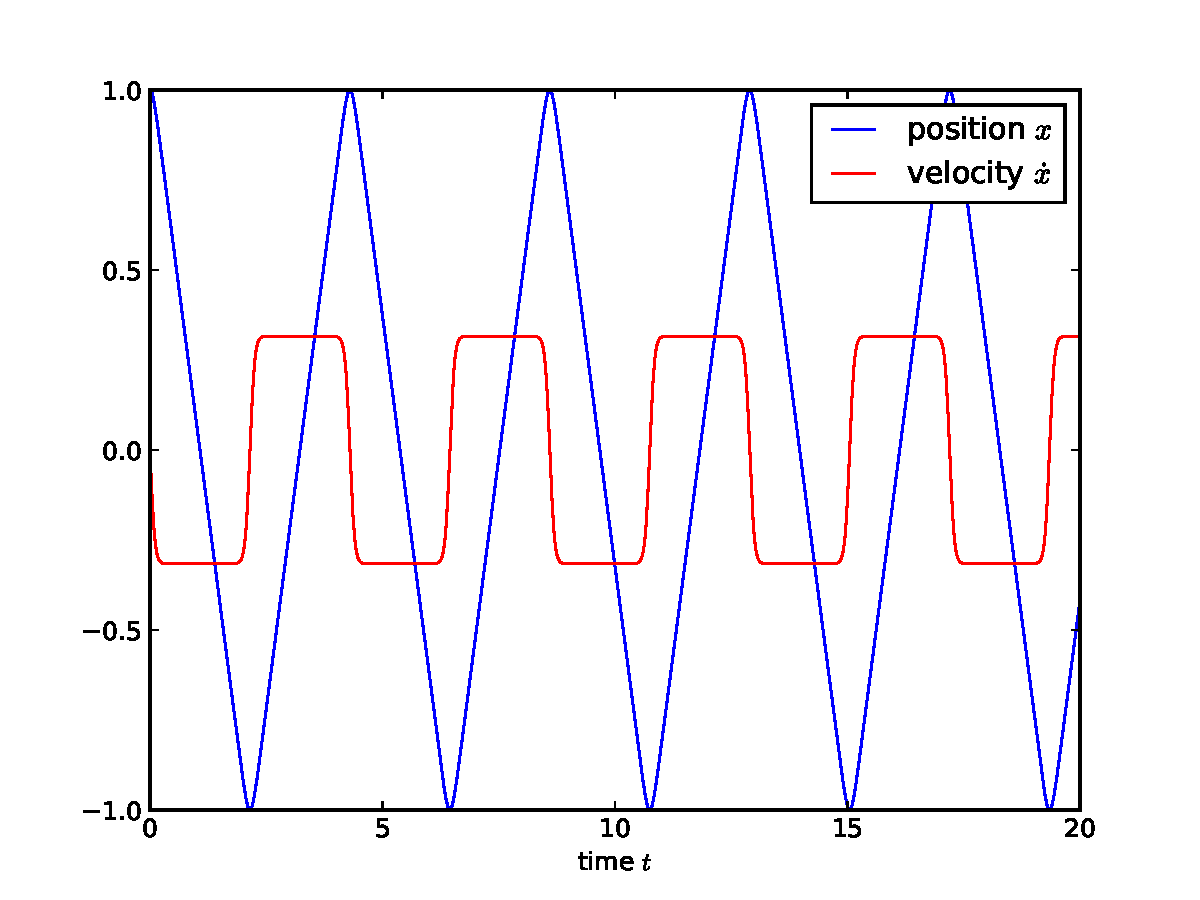
\includegraphics{./figures/anharmonic.pdf}}
\caption{numerical solutions to the anharmonic oscillator for $n=10$}
\end{center}
\end{figure}


\item \question{virial theorem in the (generalised) Kepler-problem}\\
Please simulate Kepler orbits with the script \path{kepler.py}: The equation of motion of a particle in the potential $\Phi\propto 1/r^\alpha$ can be derived from the Lagrange density
\begin{equation}
\mathcal{L} = \frac{1}{2}\left(\dot{r}^2+r^2\dot{\varphi}^2\right) + \frac{GM}{r^\alpha}
\end{equation}
Please derive the equation of motion with the Euler-Lagrange-equations and convert the resulting second-order equations in a set of first coupled order equations.

\begin{enumerate}[(a)]
\item{Change the total energy of the planet by setting $\delta$ to a value unequal to 0 and observe the change in the orbit. The product constants $GM$ is set to $GM=1$ for the numerics.}
\item{Change the value of $\alpha$ to a number different from 1: Are the orbits still closed? NB: The problem becomes unstable if $\alpha$ is too large, try to experiment in the range $\alpha=0.8\ldots1.2$.}
\item{Can you generate precession motion and orbits lagging behind by choosing a suitable $\alpha$?}
\item{Is it possible to have bound systems for $\alpha\geq 2$? What's the physical reason?}
\item{What's the virial relationship and how does it depend on $\alpha$?}
\end{enumerate}

\begin{figure}[h]
\begin{center}
\resizebox{7.5cm}{!}{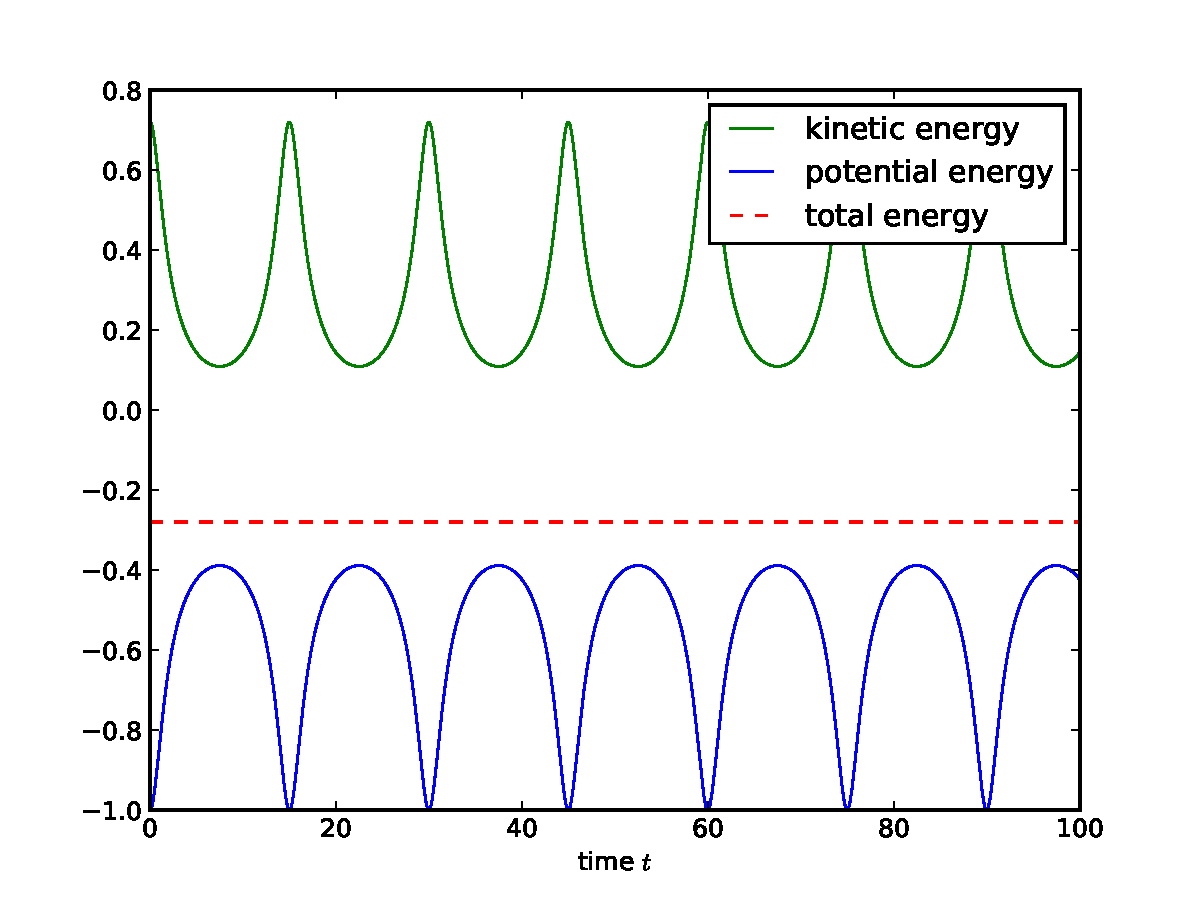
\includegraphics{./figures/kepler.pdf}}
\caption{kinetic and potential energy in Kepler-orbits}
\end{center}
\end{figure}


\end{enumerate}
\end{document}
